%% 
%%  This file is prtec-template.tex, a template for extended abstracts submitted to the
%%  Pacific Rim Thermal Engineering Conference (PRTEC).
%%
%%  PRTEC uses A4 paper.
%%
%%  This file is version 1.04 dated 2019/04/17
%%
%%  Author: John H. Lienhard V
%%          Department of Mechanical Engineering
%%          Massachusetts Institute of Technology
%%          Cambridge, MA 02139-4307 USA
%%
%%  Most of the text content is directly taken from the WORD template for this conference.
%%
%%  Class options are described in the prtec.cls file. These include:
%%
%%          * math options from M. Sharpe's newtxmath package: upright integrals [upint]; and
%%          *    [varvw] for a v and w that are better distinguished from greek nu; and also 
%%          *    [smallerops, varg, slantedGreek, frenchmath, varbb, cmbraces].
%%          *    For best results, be sure your system has v1.5 or later of newtxmath.
%%
%%          * option to omit PRTEC footer and header [nofoot]
%%
%%          * option not to use newtxtext's superiors font for footnotes [nodefaultsups] and option
%%          *    for slightly larger small capitals [largesc]
%%
%%  For details of newtxmath and newtxtext, see the documentation available on CTAN (http://ctan.org)
%%
%%  The booktabs, array, and dcolumn packages are loaded by default; those macros may be used for setting tables.
%%
 %=========================================================
%% 
%% LICENSE:
%%
%% Copyright (c) 2019 John Lienhard
%%
%% Permission is hereby granted, free of charge, to any person obtaining a copy of this software and 
%% associated documentation files (the "Software"), to deal in the Software without restriction, 
%% including without limitation the rights to use, copy, modify, merge, publish, distribute, sublicense, 
%% and/or sell copies of the Software, and to permit persons to whom the Software is furnished to do so, 
%% subject to the following two conditions:
%%
%% The above copyright notice and this permission notice shall be included in all copies or 
%% substantial portions of the Software.
%%
%% The software is provided "as is", without warranty of any kind, express or implied, including but 
%% not limited to the warranties of merchantability, fitness for a particular purpose and noninfringement. 
%% in no event shall the authors or copyright holders be liable for any claim, damages or other liability, 
%% whether in an action of contract, tort or otherwise, arising from, out of or in connection with the 
%% software or the use or other dealings in the software.
%%
%%%%%%%%%%%%%%%%%%%%%%%%%%%%%%%%%%%%%%%%%%%%%%%%%%%%%%%%%%%%%%%%%%%%%%%%%%%%%%%%%%%%%%%%%%%%%%%%%%%%%%%


%% Class options are described above.

\documentclass[upint,varvw]{prtec}

%%%%%%%%%%%%%%%%%%%%%%%%%%%%%%%%%
%% Editing tools; can delete these if not using.

\usepackage{lipsum}  % makes paragraphs of "latin" for layout testing
\usepackage{comment} % see package documentation. Can comment out sections as needed.

%%%%%%%%%%%%%%%%%%%%%%%%%%%%%%%%%%


%%%%%  pdf metadata %%%%%%%%%%%%%%%%%%%%%%%%%%%%%%%%%%%%%%%%%%%%%%%%%%%%%%%%%%%%%%%%%%%%%%%%%%%%%%%%%%%%
%%%%%  add or edit as desired

\hypersetup{%
	colorlinks=true,%%% <=== change to false to get black colored links if desired
	linkcolor=blue, %
	citecolor=blue, % SeaGreen4,%
	urlcolor=blue,  % Red3,%
	pdftitle={},    % <=== add your paper title
	pdfkeywords={}, % <=== add your keywords
	pdfauthor={},   % <=== add your name[s]
}

%%%%%%%%%%%%%  END PREAMBLE  %%%%%%%%%%%%%%%%%%%%%%%%%%%
%%%%%%%%%%%%%%%%%%%%%%%%%%%%%%%%%%%%%%%%%%%%%%%%%%%%%%%%

\begin{document}

%%%%%  Conference, title, authors, affiliations %%%%%%%%

\confname{Extended Abstracts of The Second Pacific Rim Thermal Engineering Conference}
\confdate{December 13-17, 2019}
\confcity{Maui, Hawaii, USA}

%%% Your paper number
\paperno{PRTEC-XXXXX}

%%% Your title
\papertitle{Our research paper: the latest developments in cutting-edge engineering}
 
 
%%   Put author names into the order you want. Use the same order for affiliations.
%%   \affil{#} tags the author's affiliation to the address in \SetAffiliation{#}.
%%   No space between last name and \affil{#}, separate names with commas.
%%
%%   \CorrespondingAuthor{email} follows that author's affiliation, no spaces.  
%%   If multiple corresponding authors, put both email addresses in the same command and place after both authors.
%%
%%   \JointFirstAuthor, if applicable, follows the affiliation of the relevant authors, no spaces.

\SetAuthors{Mamoru Tanahashi\affil{1}\JointFirstAuthor , Yongchan Kim\affil{2}\JointFirstAuthor , Sumanta Acharya\affil{3} , Koji Fukagata\affil{4}, John Lienhard\affil{5}\CorrespondingAuthor{lienhard@mit.edu}}

\SetAffiliation{1}{Department of Mechanical Engineering, Tokyo Institute of Technology, Japan}
\SetAffiliation{2}{School of Mechanical Engineering, Korea University, Republic of Korea}
\SetAffiliation{3}{The Mechanical, Materials, and Aerospace Engineering Department, Illinois Institute of Technology, USA}
\SetAffiliation{4}{Department of Mechanical Engineering, Keio University, Japan}
\SetAffiliation{5}{Massachusetts Institute of Technology, Cambridge, MA 02139-4307 USA}


%% Leave these two commands after title, authors, affiliations
\MakeTitlePage
\SetAuthorBlock

%%%%%%%%%%%%%%%%%%%


\begin{abstract}

This guide has been prepared for authors of extended abstract to be presented at The Second Pacific Rim Thermal Engineering Conference (PRTEC2019), December 13--17, 2019, Maui, Hawaii, USA. Authors are requested to follow these guidelines to achieve uniformity in the presentation of the proceedings. The main format of the extended abstract is as follows. Text: Times New Roman (or equivalent), 11 pt, left and right justified. Headings: Times New Roman, all capitals, 12 pt, centered. Page size A4 (210 $\times$ 297 mm); 20 mm borders all round; paper title starts at 40 mm from the top of the page except for the first page. Convert the manuscript to a single PDF file and submit it to the Online Submission System (\url{https://www.jsme.or.jp/ted/PRTEC2019/}) by the electrical format. The abstract should summarize the key findings in your study and should be in a single paragraph no more than 250 words. It should give an account of the most relevant contributions of the paper. It is also important to briefly indicate the goal, the methods, the results, and the conclusions. Avoid abbreviations, diagrams, and references. It must be self-contained and understandable without reference to the text.

\keywords{PRTEC, Extended Abstract, Template; 10 pt Times font} %% <=== Change to your keywords, keep this command before \end{abstract}.

\end{abstract}


\section{Introduction \NoCaseChange{(Details for submitting extended abstract)}}

The Extended Abstract must be formatted using this template and submitted by \textbf{June 30, 2019} for review. \textbf{The final version of the Extended Abstract must be submitted by August 31, 2019 for inclusion in the proceedings.} The final version of the extended abstract that does not conform to the correct format will not be included in the proceedings. There will be no opportunity to alter it after the submission of the final version.

It is assumed that the corresponding author will make a presentation at the conference. Each accepted extended abstract must have at least one paid regular or student registration by \textbf{August 31, 2019} to ensure that their presentation is included in the Conference Program. 


\section{Length and Layout}

The extended abstract should be in \textbf{2--5} pages in A4 size (210 $\times$ 297 mm) including tables, figures and references. The extended abstract may include color figures. The file size should not exceed 4 Mbytes after conversion to a PDF file. 

The layout of the extended abstract should follow the style of this document, starting with the title, name(s) of author(s) and affiliation(s). Put a blank line between paragraphs.

\textbf{Title:} The title should appear 40 mm below the top edge of the page.  It should be brief, clear and descriptive. Use Times New Roman 14 pt. all bold capital letters (except if formulae or symbols appear in the title), centered on the width of the typing area. Authors' names should be in lower-case letters in bold and the affiliations should be in no bold.

\textbf{ABSTRACT:} A brief abstract (100--250 words) should appear beneath the affiliation of the author(s). It should give an account of the most relevant contributions of your study. It is also important to indicate briefly the goal, the methods, the results, and conclusions. Avoid abbreviations, diagrams, and references. It must be complete and understandable without reference to the text. Leave a blank line between the Author's affiliation and the Abstract. Leave a blank line between the abstract and keywords.

\textbf{KEYWORDS:} Keywords can be selected to describe the feature of the extended abstract. Leave two blank lines between keywords and the first major heading.

\textbf{Header and footnotes:} The header includes the Paper number. \textbf{Please insert your presentation ID supplied by the Online Submission System, e.g., PRTEC-23456, if your presentation ID is PRTEC-23456.} The footnote of the first page contains E-mail address of the corresponding author. Note that this ``formal'' corresponding author can be different from the ``practical'' corresponding author registered on the submission system. Do not edit the copyright line. We do not transfer the copyright for the authors' convenience. The copyright line should always appear as ``Copyright \textcopyright\ 2019 by The Author(s). Distributed by JSME, KSME, and ASTFE with permission.'' Do not substitute the authors' names in the copyright line.



\section{Headings and Equations}

If your extended abstract is divided into sections and subsections, please use the format adopted here, in which the first-level headings are in 12 pt bold capitals, centered. Put two blank lines before the heading and a blank line after the heading.

\subsection{Second-Level Headings}  The second-level headings should be in 12 pt bold lower case (initial capital), left aligned.

\subsubsection{Third-level headings} The third-level headings should be placed at the beginning of a paragraph. Capitalize only the first letter of the whole subhead ended with a period and underline it (if possible, make the subhead italic). With two-letter spacing, begin typing the text on the same line and continue the text without indenting again. Leave one line space above.

Equations should be typed in position with an appropriate space above and below to distinguish them from the text. Use common fonts like Times New Roman in your math equations. Do not insert equations in a non-editable picture format. All equations should be numbered, \textit{e.g.}, 
\begin{equation}
\dot{r}(\alpha) = \lambda
\end{equation}
and
\begin{equation}
k_{ij} = \theta_1\exp\left(-\frac{1}{2}\sum_{d=1}^D \frac{(x_i-x_j)^2}{\lambda_d^2}\right).
\end{equation}

An equation is a part of the text: do not isolate the equation. Put relevant punctuations. The Equation number should be flush right with a line space above and below the equation. Align equal signs when 
equations are stacked with no intervening words.

Subscripts and superscripts should clearly be typed, and the manuscript should be reviewed carefully to ensure there is no ambiguity in presentation. Numbers and letters that are intended to be subscripts or superscripts should not be aligned with the rest of the text.

All data should be reported in SI units. Decimals should always be shown by periods and not by commas or centered dots.


%%%%%%%%%%%%%%%%%   figure 1    %%%%%%%%%%%%%%%%%%%%%%
\begin{figure}[tb]
\centering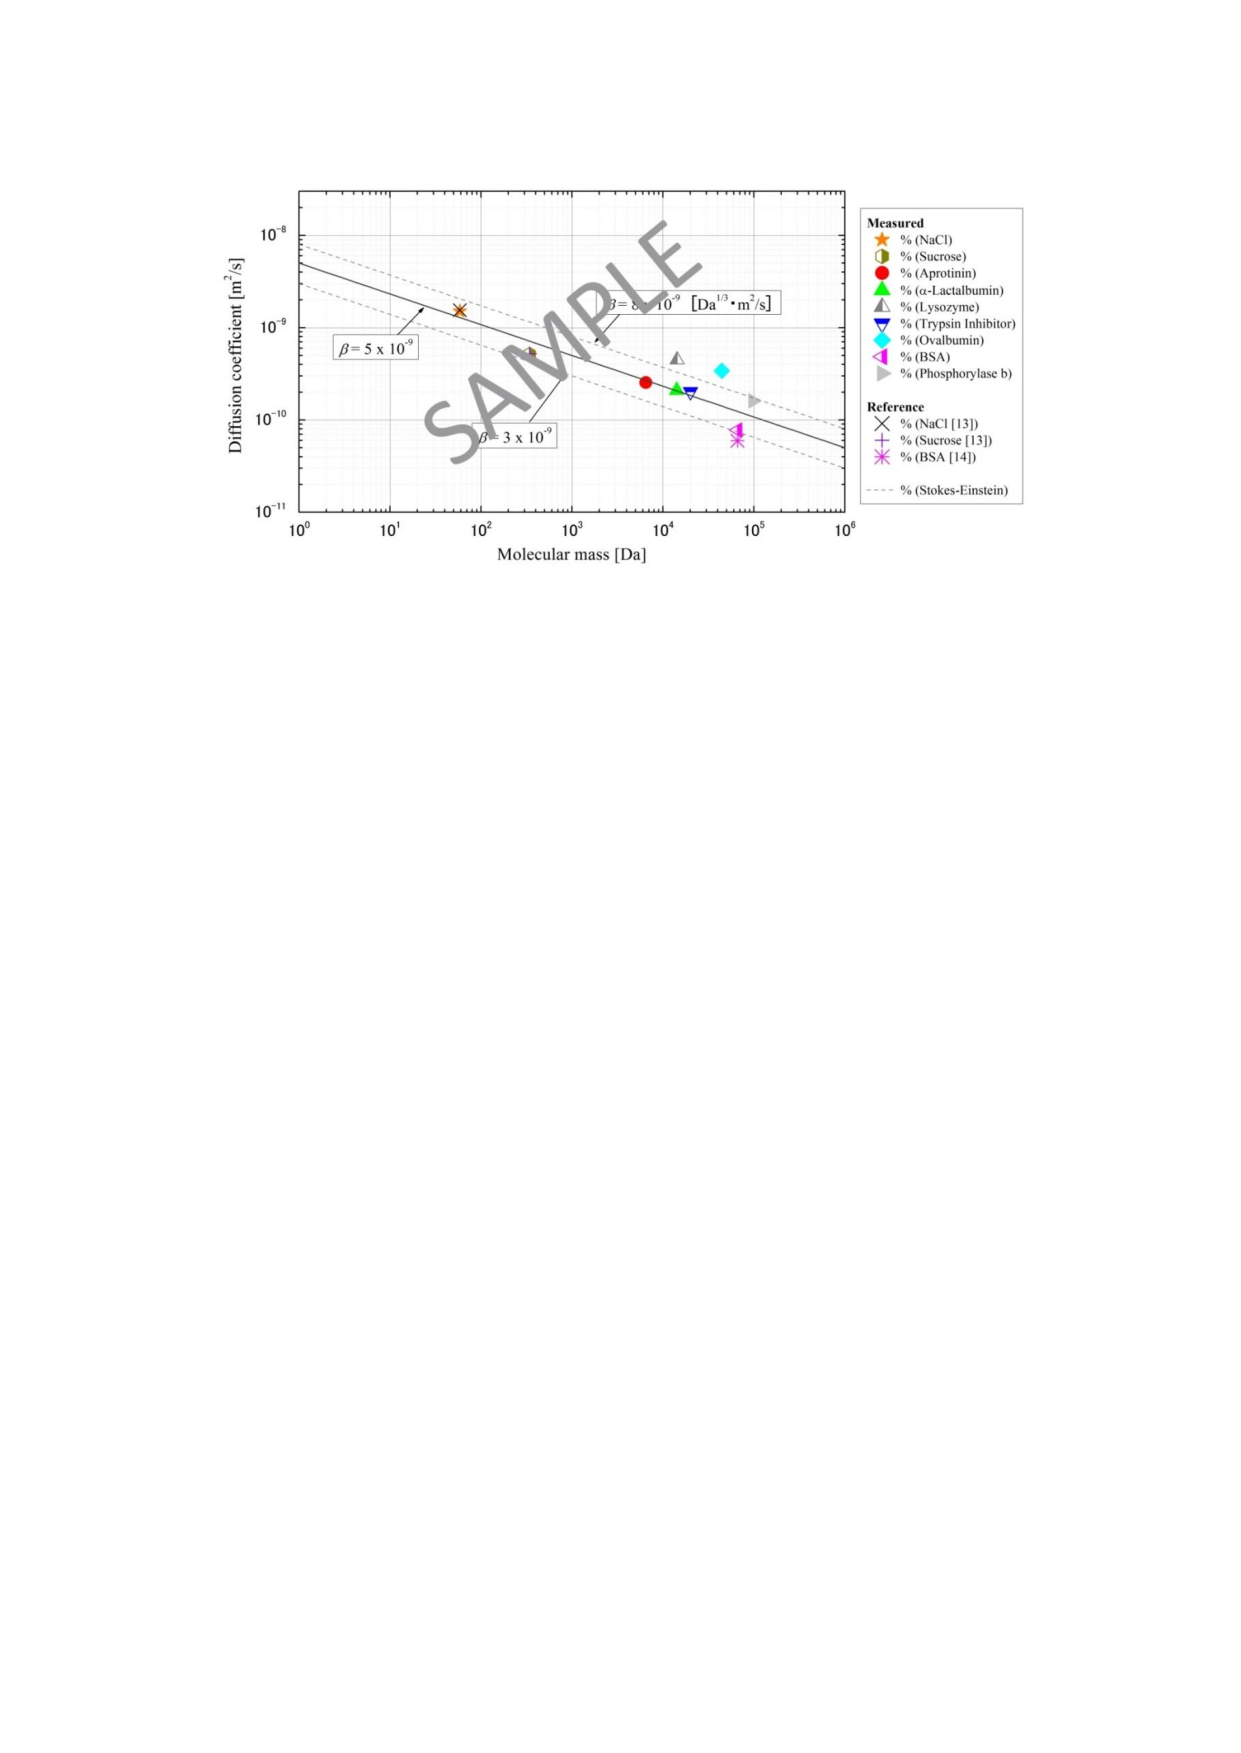
\includegraphics[width=\linewidth]{sample-figure.pdf}
\caption{\label{fig:1} One-line figure caption is centered under the figure. Make a space above the figure caption.}
\end{figure}
%%%%%%%%%%%%%%%%%%%%%%%%%%%%%%%%%%%%%%%%%%%%%%%%%%%%%%


\section{Figures and Tables}

\subsection{Figures}  Care should be taken to ensure that figures are contained within the typing area. All original drawings should be prepared. As a general rule, lettering (i.e., font type and size) in the figures should be comparable to that in the text. Color and black/white photographs are allowed in digital format with sufficient resolution to permit high-quality reproduction, and imported into the manuscript. Use or insert .jpg, .tiff, .gif, or similar program files for illustrations. Do not use PowerPoint or graphic constructions as they provide poor quality illustrations.

Figures should be numbered consecutively, and they are referred as, \textit{e.g.}, Fig.\ 1, with a single letter space between the word ``Fig.'' and the Arabic numeral, but do not abbreviate it if it appears at the beginning of a sentence; namely, not ''Fig.\ 1 shows\ldots '' but ``Figure 1 shows\ldots'' at the beginning of a sentence. 

Place figures centered on the width of the text page, either at the top or bottom of the page as close as possible to their first mentioning text. Figure captions should appear below the respective figure. Type the word ``Fig.'' and its number followed by two-letter space. Then, type the caption single spaced, with an initial capital for the first word and for proper nouns only. Provide relevant spacing around the figure.

\subsection{Tables} When tables are referred in the text, they should be referred to as Table 1, Table 5, etc.\ (\textit{i.e.}, with a single letter space between the word ``Table'' and the Arabic numeral). Separate the title from the column heads, ranks within column heads, column heads from table body, and table body from table footnotes or source. 

Place tables centered on the width of the text page, either at the top or bottom of the page as close as possible to their first mentioning text. Table captions should appear above the respective table.  Each table should have at least a two-line space both above the table and between the table and the start of the following text. 

The first  letter of the word ``Table'' should be capitalized, followed by the table number and period, then the caption with the first letter of main words capitalized, all centered above the table as shown below. Use horizontal rules above and below. Tables are in Times New Roman, 11 pt: one-line heading, centered; two- or more-line heading flush left. The table caption is placed above the table, with one line space above and below the caption. Type size of the body of the table depends on the size of the table, adjust type size accordingly.

%%%%%%%%%%%%%%% table  1  %%%%%%%%%%%%%%%%%%%  

\begin{table}[tb]
\caption{\label{tab:1} The table caption is above the table. Captions that are two or more lines are flushed left, one line space above and below the caption.}
\centering{%
\setlength{\tabcolsep}{18pt} %% three times the normal column separation (6 pt) for this table only. (Not recommended in general)
\begin{tabular}{ccccc}
\toprule
Case & Diameter $d_B$ [mm] & $f$ [Hz] & We & St \\
\midrule
1&	0.5&	731 &	117&	0.15\\
2&	0.5&	1799&	620&	0.16\\
3&	1.3&	198 &	124&	0.17\\
\bottomrule
\end{tabular}
}
\end{table}

%% The prtec class loads the booktabs package, so you can use \toprule, \midrule, \bottomrule from that package.

%%%%%%%%%%%%%%%%%%%%%%%%%%%%%%%%%%%%%%%%%%%%


\section{Non-English Speaking Authors}
Authors from non-English speaking countries are requested to find persons who are competent in English and familiar with the scientific language and can edit their manuscripts before submission.  Reviewers may not be relied on to make corrections of English expression, spelling, etc.  As there is no editing stage for publication-ready manuscripts, it is the responsibility of authors to ensure that the presentation of their extended abstracts reaches the same high level as that of the work they describe.

\section{Conclusions}
\textbf{Paper Size and Length:} A4 (210 $\times$ 297 mm) and 2--5 pages.

\textbf{Margins:} 20 mm margins all round as in the Full Paper Template.

\textbf{Line Spacing:} Single-spaced with one blank line between paragraphs. No paragraph indentation.

\textbf{Justification:} Full justification.

\textbf{Page Numbering:} Pages should be numbered.

\textbf{Figures and tables:} Figures and tables should be placed at the top or bottom of the page on which they are first mentioned if possible, on the next page if not. Do not gather them at the end of the extended abstract.

\textbf{Submission:} The Extended Abstract should be converted to a single PDF file whose size is no more than 4 Mbytes, and submitted to the Online Submission System (\url{https://www.jsme.or.jp/ted/PRTEC2019/}).

\textbf{Submission Deadline for review:} Extended Abstract for review should be submitted by \textbf{June 30, 2019}. Notification of acceptance will be made by July 15, 2019.

\textbf{Submission Deadline for final version:} All contributors must upload the final version of Extended Abstract for inclusion in the proceedings by \textbf{August 31, 2019} even if there is no modification from the initial Extended Abstract. The Final Extended Abstract that does not conform to the correct format will not be included in the proceedings.  There will be no opportunity to alter it after the submission of the final version.


\section*{Acknowledgements} 
Acknowledgments should be placed immediately following CONCLUSIONS, if necessary.


%%%%%%%%%%  Nomenclature  %%%%%%%%%%%%%%%%%%%%%%%%%

{\color{red}The editors of the major heat transfer journals have adopted a common list of symbols. The symbol list can be found in \textit{Journal of Heat Transfer}, \textbf{121}, 770-773 (1999).  All authors should use these symbols for the extended abstract submitted for this conference. \textbf{The symbols defined in this common list need not be included in the nomenclature list; only symbols unique to the extended abstract should be listed here.} A short nomenclature defining unusual or non-standard symbols should be placed immediately above the REFERENCES. SI Units must be used.}

%% omitting the second argument of \entry will format subheading (see examples)
\begin{nomenclature}
\entry{Roman letters}
\entry{Be}{dimensionless variable [--]}
\entry{$\hat{C}$}{second variable [s$^{-2}$]}
\entry{$Q_A$}{third variable [kJ]}
\entry{$w_x$}{fourth variable [m$^{2}$ s$^{-1}$]}

\entry{Greek letters}
\entry{$\zeta$}{dimensionless variable [--]}
\entry{$\phi(\Omega)$}{function [--]}
\entry{$\Omega$}{fifth variable [s$^{-1}$]}

\end{nomenclature}


%%%%%%%%%%%%%  References  %%%%%%%%%%%%%%%%%%%%%%%%%

\nocite{*} % remove this command unless you with to typeset your entire .bib file

\bibliographystyle{prtec}
\bibliography{prtec-sample} % <=== Change to the name of your .bib file



%%%%%%%%%%%%%  Appendices  %%%%%%%%%%%%%%%%%%%%%%%%
\appendix

\section{Additional notes for \LaTeX\ users}
The PRTEC class file is compatible with \hologo{pdfLaTeX}, \hologo{LuaLaTeX}, and \hologo{XeLaTeX}. The class relies on the \texttt{newtx} math and text fonts and is not configured for \texttt{fontspec}. The class will automatically set the needed margins, spacings, font sizes, and citation formats. The class is also designed to support hyperlinks, metadata, and pdf bookmarks.

The class loads the \verb|\booktabs|, \verb|\array|, and \verb|\dcolumn| packages, for use in formatting tables.

PRTEC requires that section headings be set in uppercase, bold-face type.  The class will do this automatically.  You can place \verb|\cite{..}|, \verb|\ref{..}|, \verb|\label{..}|, and into headings directly, as you would in the main text. Do not enclose them braces, e.g.\ \verb|{\cite{..}}|, which will cause errors. You can place \verb|\footnote{..}| into headings, but not into captions.\footnote{See \texttt{tex-stackexchange} for various approaches to footnotes in captions, if they seem necessary. For footnotes inside tables, use the \texttt{tablefootnote} package.}

Math in headings will automatically be set using \verb|\mathversion{bold}|. Outside of headings, for bold math you can use the \verb|\bm{..}| macro from the \texttt{bm} package, which is loaded by the class. 

Text in section headings will not be capitalized if enclosed in a \verb|\NoCaseChange{..}| command.

The pdf bookmarks are automatically set as the text of the section heading. Simple math expressions can be used in the section headings, without causing errors in the bookmarks.  For a section heading that includes more complicated math (and macros), you may use the optional argument of \verb|\section[..]{..}| to create a pdf bookmark without losing characters or producing warnings or errors. See the \texttt{prtex-template.tex} source file for an example of this, in the following section head.

%% For math in a section heading: the optional argument creates a pdfbookmark 
%%     without an error message or loss of characters.
\section[Proof that S-gen\neq 0]{Proof that $\dot{S}_{\textrm{gen}}\neq 0$}

For math in a section heading, the optional argument of \verb|\section[..]{..}| creates a pdfbookmark without losing characters or producing error messages. For this example, we use:

\verb|\section[Proof that S-gen\neq 0]{Proof that $\dot{S}_{\textrm{gen}}\neq 0$}|

Observe that some simple math expressions are accepted by the \verb|hyperref| package that manages the bookmarks.

\end{document}